\documentclass{beamer}
\usetheme{Dresden}
\usecolortheme{dove}
%% Checking if saving file is working more
%\usepackage{graphicx} %For jpg figure inclusion
%\usepackage{times} %For typeface
%\usepackage{epsfig}
\usepackage{color} %For Comments
\usepackage{beamerthemeshadow} %Paul and Lemmon put this in, take out if you want
%\usepackage[all]{xy}
%\usepackage{float}
%\usepackage{subfigure} 
%\usepackage{hyperref}
%\usepackage{url}
%\usepackage{parskip}
%\usepackage{multirow}

\definecolor{ForestGreen}{RGB}{34,139,34}
\definecolor{BestBlue}{RGB}{80,255,255}
% Uncomment this if you want to show work-in-progress comments
\newcommand{\comment}[1]{{\bf \tt  {#1}}}
% Uncomment this if you don't want to show comments
%\newcommand{\comment}[1]{}
\newcommand{\emcomment}[1]{\textcolor{ForestGreen}{\comment{Elena: {#1}}}}
\newcommand{\todo}[1]{\textcolor{blue}{\comment{To Do: {#1}}}}
\newcommand{\thcomment}[1]{\textcolor{BestBlue}{\comment{Thomas: {#1}}}}
\newcommand{\rmcomment}[1]{\textcolor{magenta}{\comment{Ryan: {#1}}}}
%%%%%%%%%%%%%%%%%%%%%%%%%%%%%%%%%%%%%%%%%%

\begin{document}
\author{Elena Machkasova, Thomas Hagen, Ryan McArthur}
\title{Super-fun with First-class Shapes in Quil}
\date{November 16, 2015}


\begin{frame}
\frametitle {Super-fun with First-class Shapes in Quil}
\maketitle
\end{frame}
%frame

\begin{frame}
\frametitle{Table of contents}
\tableofcontents  
\end{frame}

\section{Who we are and why we are here}

\begin{frame}
\frametitle{Where are we from?}
\begin{figure}[h]

\includegraphics[width=7cm]{PresentationImages/umm-winter.jpg}
\end{figure}
UMM is a small liberal arts campus of UMN located 3 hours driving from Minneapolis/St.Paul. 
\end{frame}

\begin{frame}
\frametitle{What are we working on?}
Developing Clojure-based introductory CS course ({\it \href{http://cda.morris.umn.edu/~elenam/\#clojure}{ClojurEd project}}). 

What does this include? 
\begin{enumerate}
\item Beginner-friendly error messages. 
\item Libraries and tools that allow beginners to explore functional approaches, recursion, and abstraction.
\item Integration into a beginner-friendly IDE. 
\end{enumerate}
\end{frame}

\begin{frame}
\frametitle{What are we working on?}
Developing Clojure-based introductory CS course ({\it \href{http://cda.morris.umn.edu/~elenam/\#clojure}{ClojurEd project}}). 

What does this include? 
\begin{enumerate}
\item Beginner-friendly error messages. 
\item {\bf Libraries and tools that allow beginners to explore functional approaches, recursion, and abstraction: graphical library.}
\item Integration into a beginner-friendly IDE. 
\end{enumerate}
Summer project 2015. 
\end{frame}

\begin{frame}[fragile]
\frametitle{Beginner-friendly graphical library}
Inspiration: Racket "universe" package (MVC, first-class shapes):
\begin{verbatim}
(define (main duration)
  (big-bang '() ; starts with an empty list of positions.
   [to-draw display-dots] ;draw dots on canvas
   [on-tick do-nothing 1 duration] ;dots don't move w/time
   [on-mouse add-or-remove-dot])) ;click handling
\end{verbatim}
\begin{figure}[h]
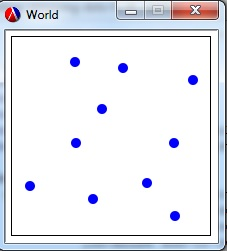
\includegraphics[width=4cm]{PresentationImages/dots.jpg}
\end{figure}
\end{frame}

\begin{frame}[fragile]
\frametitle{Beginner-friendly graphical library}
\begin{verbatim}
(define dot (circle 10 "solid" "blue"))

;; display-dots: list of positions  -> image
(define (display-dots lop)     
  (cond [(empty? lop) blank-scene]
        [else (place-image dot
                           (posn-x (first lop))
                           (posn-y (first lop))
                           (display-dots (rest lop)))]))

;; add-or-remove-dot: list of positions, 
;; coordinates of click -> list of positions
.........
\end{verbatim}

\end{frame}

\begin{frame}
\frametitle{Odds and ends (not an actual slide)}
\emcomment{Don't forget:
\begin{enumerate}
\item Mention Racket influence  
\item Mention the author of Quil fun mode
\item Mention Tom Hall EuroClojure 2014
\end{enumerate}
}
\end{frame}



\begin{frame}
\frametitle{Shapes as First Class Objects}
\thcomment{like racket. Wanted to have shape object. collage style.}
	\begin{itemize}
		\item Racket-style implementation of shapes
		\item Shapes are treated as objects, modified through functions
		\item Shapes hold their specifications for drawing
		\item Easy to redraw wherever needed
		\item Easier to understand conceptually for students
	\end{itemize}
\end{frame}

\begin{frame}


\frametitle{Simple Shapes}
\thcomment{create shape template, then reuse when needed. Quil does it this way (ex)}
	\begin{itemize}
		\item Quil shapes live in the draw function
		\item Quil shapes are functions to draw the shape
	\end{itemize}
	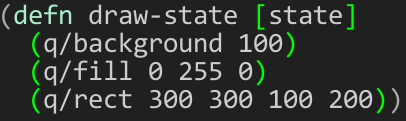
\includegraphics[width=4cm]{PresentationImages/quilGreenRect.png}
\end{frame}

\begin{frame}
\frametitle{Our Shapes}
\thcomment{We do it this way (ex). Uses draw function.}
	\begin{itemize}
		\item Our shapes are defined once and reused when needed
		\item Our shapes are drawn through the draw-shape (or ds) function
	\end{itemize}
	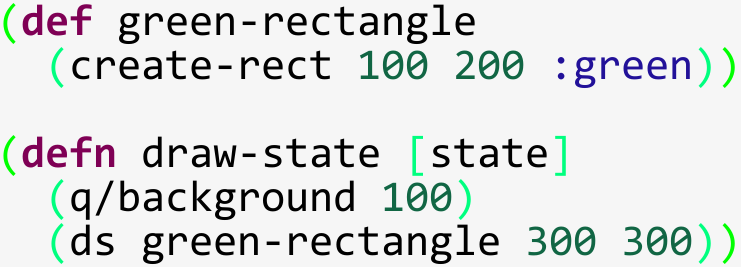
\includegraphics[width=4cm]{PresentationImages/fcsGreenRect.png}
\end{frame}

\begin{frame}
\frametitle{Creating a Collage}
\thcomment{We do it this way (ex). Uses draw function.}
	\begin{itemize}
		\item Functional Quil uses paintbrush approach
		\item Our firstclass-shapes use collage approach
	\end{itemize}
\thcomment{Talk about mvc differences here, get Elena to word it}
\end{frame}

\begin{frame}
\frametitle{Complex Shapes}
\thcomment{creating complex shapes. deconstructable.}
	\begin{itemize}
		\item Complex shapes are a collection of simple shapes
		\item Each simple shape holds their individual offsets
		\item Methods are used to create complex shapes from simple ones
	\end{itemize}
	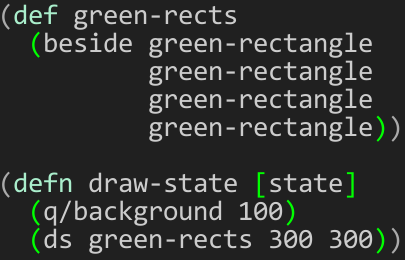
\includegraphics[width=4cm]{PresentationImages/fcsGreenRects.png}
	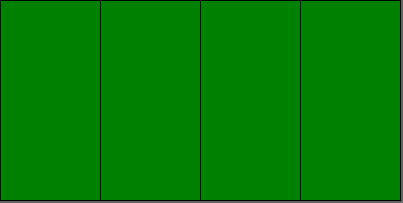
\includegraphics[width=4cm]{PresentationImages/4GreenRects.png}
\end{frame}

\begin{frame}
\frametitle{Above and Beside}
\thcomment{show above and beside (ex)}
	\begin{itemize}
		\item Complex shapes are constructed through calling above or beside
		\item Can use reduce and map
	\end{itemize}
	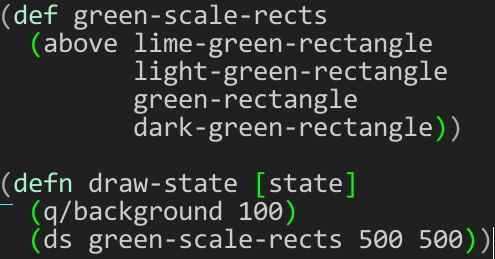
\includegraphics[width=4cm]{PresentationImages/greenScaleRects.png}
	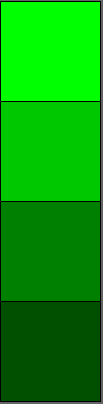
\includegraphics[width=1cm]{PresentationImages/greenScaleTower.png}
\end{frame}

\begin{frame}
\frametitle{Overlay}
\rmcomment{show overlay}
	\begin{itemize}
		\item Complex shapes are also constructed through overlay
	\end{itemize}
	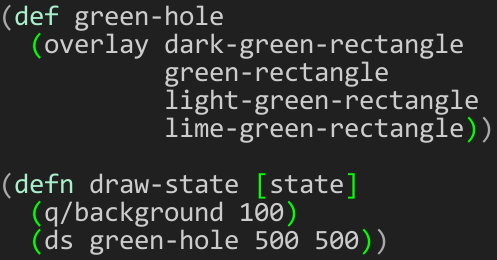
\includegraphics[width=4cm]{PresentationImages/fcsGreenHoleCode.png}
	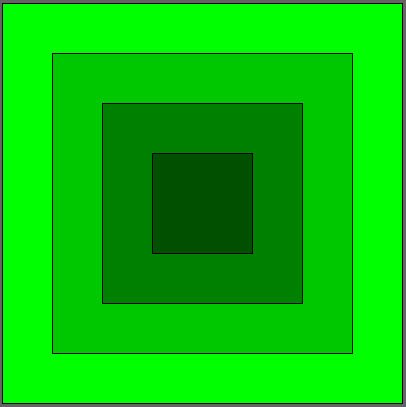
\includegraphics[width=4cm]{PresentationImages/greenHole.png}
\end{frame}

\begin{frame}
\frametitle{Align}
\rmcomment{beside align overlay align etc. (ex)}
	\begin{itemize}
		\item An align version of overlay, above, and beside exist
	\end{itemize}
	
\includegraphics[width=1cm]{PresentationImages/greenLeanRight.png}
	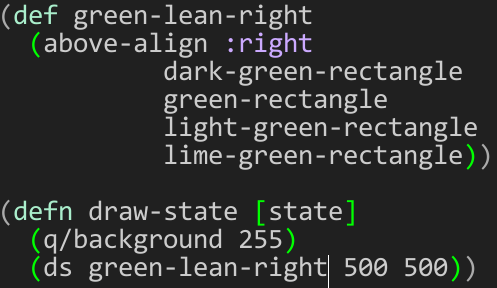
\includegraphics[width=3cm]{PresentationImages/greenLeanRightCode.png}
	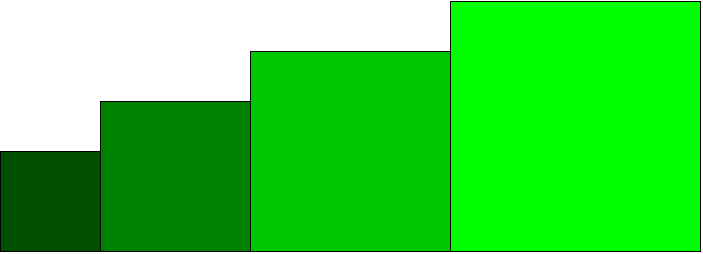
\includegraphics[width=1cm]{PresentationImages/greenSlopeBottom.png}
	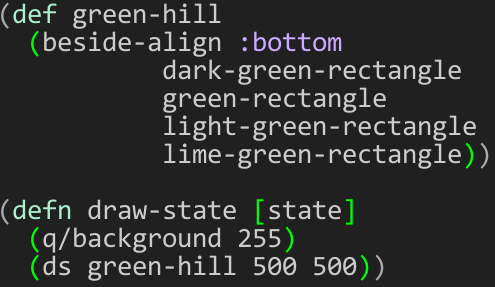
\includegraphics[width=3cm]{PresentationImages/greenSlopeBottomCode.png}
	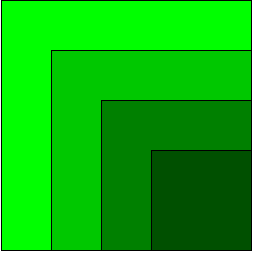
\includegraphics[width=1cm]{PresentationImages/greenAlignBottomRight.png}
	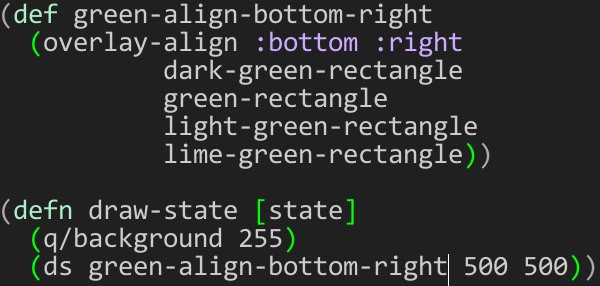
\includegraphics[width=3cm]{PresentationImages/greenAlignBottomRightCode.png}
\end{frame}

\begin{frame}[fragile]
\frametitle{Rotation and Scaling}
	\begin{itemize}
	\item You can modify the size and orientation of the shape
	\begin{columns}[t]
		\begin{column}{.45\textwidth}
			\begin{figure}[h]
			
\includegraphics[width=4cm]{PresentationImages/rotateRedCode.png}
			\end{figure}
		\end{column}
		\begin{column}{.3\textwidth}
			\begin{figure}[h]
			
\includegraphics[width=0.8cm]{PresentationImages/red-rectangle-rotate.png}
			\end{figure}		
		\end{column}
		\end{columns}
		
		\begin{columns}[t]
		\begin{column}{.45\textwidth}
			\begin{figure}[h]
			
\includegraphics[width=4cm]{PresentationImages/scaleRedCode.png}
			\end{figure}
		\end{column}
		\begin{column}{.3\textwidth}
			\begin{figure}[h]
			
\includegraphics[width=1.2cm]{PresentationImages/red-rectangle-scale.png}
			\end{figure}		
		\end{column}
		\end{columns}
		
		\begin{columns}[t]
		\begin{column}{.45\textwidth}
			\begin{figure}[h]
			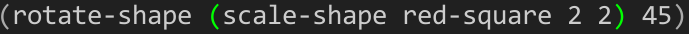
\includegraphics[width=6.5cm]{PresentationImages/rotateAndScaleRedCode.png}
			\end{figure}
		\end{column}
		\begin{column}{.3\textwidth}
			\begin{figure}[h]
			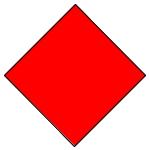
\includegraphics[width=1.7cm]{PresentationImages/red-rectangle-scale-rotate.png}
			\end{figure}		
		\end{column}
		\end{columns}
	\end{itemize}
\end{frame}


\begin{frame}
\frametitle{Images}
\thcomment{images treated like shapes. Rotate, applying most of the functions.}
	\begin{itemize}
		\item images can be rotated and scaled similar to shapes
	\end{itemize}
	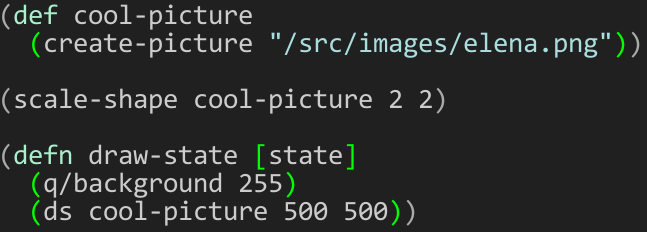
\includegraphics[width=4cm]{PresentationImages/pictureCode.png}
	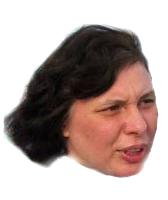
\includegraphics[width=1.7cm]{PresentationImages/elena.png}
\end{frame}

\thcomment{Put Beach example here}

\begin{frame}
\frametitle{Implementation}
\rmcomment{to do}
\end{frame}

\begin{frame}
\frametitle{Simple Shape Structure}
\rmcomment{Explain how the shape structure is set up.}
	\begin{itemize}
		\item As a data structure, simple shapes are hash's
		\item Shapes hold a variety of information within them
	\end{itemize}
	\thcomment{Hash example here}
\end{frame}

\begin{frame}
\frametitle{Complex Shape Structure}
\rmcomment{Explain the complex shape structure}
	\begin{itemize}
		\item Complex shapes are vectors of shapes
		\item Each shape knows its position from the core of the shape
		\item This allows for a 'deconstructable' complex shape
	\end{itemize}
	\thcomment{explode example here}
\end{frame}

\begin{frame}
\frametitle{Draw-Shape Structure}
\rmcomment{Explain how the draw-shape function works.}
	\begin{itemize}
		\item Draw-shape calls the internal Quil draw function within the shape object
		\item Draw-shape also works on image objects
	\end{itemize}
\end{frame}

\begin{frame}
	\frametitle{Future Work}
	\begin{itemize}
		\item Fill out more functionality
		\begin{itemize}
			\item Rotate more complex shapes
			\item Pixel-detail Overlay and Overlay-Align
			\item More seamless integration with Quil fun-mode
		\end{itemize}
		\item Open Source the project \emcomment{Done?}
		\item Integrate a Clojure sound library
	\end{itemize}
\end{frame}

\begin{frame}
\frametitle{Acknowledgments}
\emcomment{Need proper acknowledgments and logos; also probably thank Cognitect and other conj sponsors for providing an opportunity to talk}
	Our research was sponsored by:
	\begin{itemize}
	\item HHMI
	\item LSAMP
	\end{itemize}
	{\centering
	\noindent
	Thank you! \par
	Any questions? \par
	}
\end{frame}
\end{document}